\PassOptionsToPackage{unicode=true}{hyperref} % options for packages loaded elsewhere
\PassOptionsToPackage{hyphens}{url}
%
\documentclass[]{article}
\usepackage{multicol}
\usepackage{CJKutf8}
\usepackage{lmodern}
\usepackage{amssymb,amsmath}
\usepackage{ifxetex,ifluatex}
\usepackage{fixltx2e} % provides \textsubscript
\ifnum 0\ifxetex 1\fi\ifluatex 1\fi=0 % if pdftex
  \usepackage[T1]{fontenc}
  \usepackage[utf8]{inputenc}
  \usepackage{textcomp} % provides euro and other symbols
\else % if luatex or xelatex
  \usepackage{unicode-math}
  \defaultfontfeatures{Ligatures=TeX,Scale=MatchLowercase}
\fi
% use upquote if available, for straight quotes in verbatim environments
\IfFileExists{upquote.sty}{\usepackage{upquote}}{}
% use microtype if available
\IfFileExists{microtype.sty}{%
\usepackage[]{microtype}
\UseMicrotypeSet[protrusion]{basicmath} % disable protrusion for tt fonts
}{}
\IfFileExists{parskip.sty}{%
\usepackage{parskip}
}{% else
\setlength{\parindent}{0pt}
\setlength{\parskip}{6pt plus 2pt minus 1pt}
}
\usepackage{hyperref}
\hypersetup{
            pdfborder={0 0 0},
            breaklinks=true}
\urlstyle{same}  % don't use monospace font for urls
\usepackage{longtable,booktabs}
% Fix footnotes in tables (requires footnote package)
\IfFileExists{footnote.sty}{\usepackage{footnote}\makesavenoteenv{longtable}}{}
\usepackage{graphicx,grffile}
\makeatletter
\def\maxwidth{\ifdim\Gin@nat@width>\linewidth\linewidth\else\Gin@nat@width\fi}
\def\maxheight{\ifdim\Gin@nat@height>\textheight\textheight\else\Gin@nat@height\fi}
\makeatother
% Scale images if necessary, so that they will not overflow the page
% margins by default, and it is still possible to overwrite the defaults
% using explicit options in \includegraphics[width, height, ...]{}
\setkeys{Gin}{width=\maxwidth,height=\maxheight,keepaspectratio}
\setlength{\emergencystretch}{3em}  % prevent overfull lines
\providecommand{\tightlist}{%
  \setlength{\itemsep}{0pt}\setlength{\parskip}{0pt}}
\setcounter{secnumdepth}{0}
% Redefines (sub)paragraphs to behave more like sections
\ifx\paragraph\undefined\else
\let\oldparagraph\paragraph
\renewcommand{\paragraph}[1]{\oldparagraph{#1}\mbox{}}
\fi
\ifx\subparagraph\undefined\else
\let\oldsubparagraph\subparagraph
\renewcommand{\subparagraph}[1]{\oldsubparagraph{#1}\mbox{}}
\fi
\usepackage[left=0.5in, right=0.5in, bottom=1.0in, top=1.0in]{geometry}
% set default figure placement to htbp
\makeatletter
\def\fps@figure{htbp}
\makeatother


\date{}

\begin{document}
\begin{CJK*}{UTF8}{bsmi}
\hypertarget{header-n0}{%
\section{Digital Signal Processing Homework 1}\label{header-n0}}

\hypertarget{header-n3}{%
\subsection{Discrete Hidden Markov Model Implement       b05901033 電機三 莊永松}\label{header-n3}}

\hypertarget{header-n4}{%
\subsubsection{Environment}\label{header-n4}}

\begin{verbatim}
OS: Ubuntu 16.04.5 LTS (GNU/Linux 4.15.0-36-generic x86_64)
Compiler: g++ (Ubuntu 5.4.0-6ubuntu1~16.04.10) 5.4.0 20160609
CPU: Intel(R) Xeon(R) CPU E5-1620 v3 @ 3.50GHz
RAM: 32G
\end{verbatim}

\hypertarget{header-n6}{%
\subsection{How to execute?}\label{header-n6}}

\begin{itemize}
\item
  Use the command \texttt{make} to compile executable files
  \texttt{train} \texttt{test} \texttt{accuracy}, use
  \texttt{make\ clean} to remove all compiled files.
\item
  Train:
  \texttt{./train\ {[}iteration{]}\ {[}initial\ model\ file{]}\ {[}sequence\ file{]}\ {[}output\ file{]}}
\item
  Test:
  \texttt{./test\ {[}model\ list{]}\ {[}sequence\ file{]}\ {[}output\ file{]}}
\item
  Compute Accuracy:
  \texttt{./accuracy\ {[}predict\ file{]}\ {[}answer\ file{]}\ {[}output\ file{]}}
\end{itemize}

\hypertarget{header-n16}{%
\subsection{Some Analysis}\label{header-n16}}

\hypertarget{header-n17}{%
\subsubsection{Relation between accuracy and
iteration}\label{header-n17}}

\begin{longtable}[]{ll}
\toprule
iteration & accuracy\tabularnewline
\midrule
\endhead
% 0 & 0.1992 & 200 & 0.8524\tabularnewline
% 1 & 0.7660 & 300 & 0.8488\tabularnewline
% 5 & 0.6484 & 400 & 0.8536\tabularnewline
% 10 & 0.5408 & 500 & 0.8556\tabularnewline
% 15 & 0.6104 & 600 & 0.8632\tabularnewline
% 20 & 0.7904 & 700 & 0.8664\tabularnewline
% 50 & 0.8228 & 800 & 0.8684\tabularnewline
% 100 & 0.8104 & 900 & 0.8696\tabularnewline
% 150 & 0.8600 & 1000 & 0.8700\tabularnewline
0 & 0.1992\tabularnewline
1 & 0.7660\tabularnewline
5 & 0.6484\tabularnewline
10 & 0.5408\tabularnewline
15 & 0.6104\tabularnewline
20 & 0.7904\tabularnewline
50 & 0.8228\tabularnewline
100 & 0.8104\tabularnewline
150 & 0.8600\tabularnewline
200 & 0.8524\tabularnewline
300 & 0.8488\tabularnewline
400 & 0.8536\tabularnewline
500 & 0.8556\tabularnewline
600 & 0.8632\tabularnewline
700 & 0.8664\tabularnewline
800 & 0.8684\tabularnewline
900 & 0.8696\tabularnewline
1000 & 0.8700\tabularnewline
\bottomrule
\end{longtable}
\clearpage
\hypertarget{header-n76}{%
\subsubsection{Visualization}\label{header-n76}}

\begin{figure}
\centering
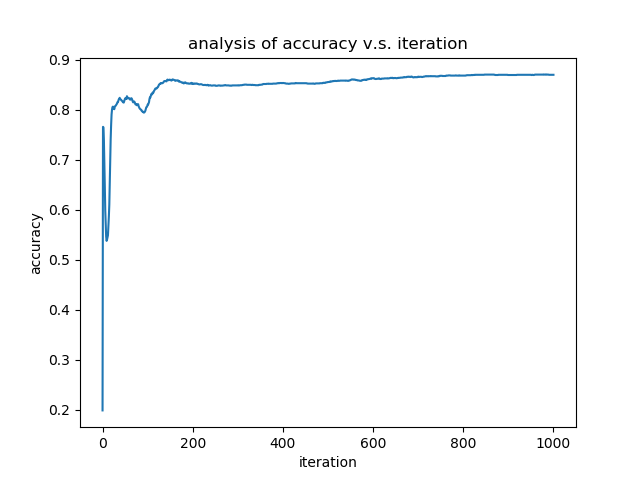
\includegraphics[width=10cm, height=13.33cm]{ana.png}
\caption{}
\end{figure}

\hypertarget{header-n78}{%
\subsubsection{Use log scale for iteration axis}\label{header-n78}}

\begin{figure}
\centering
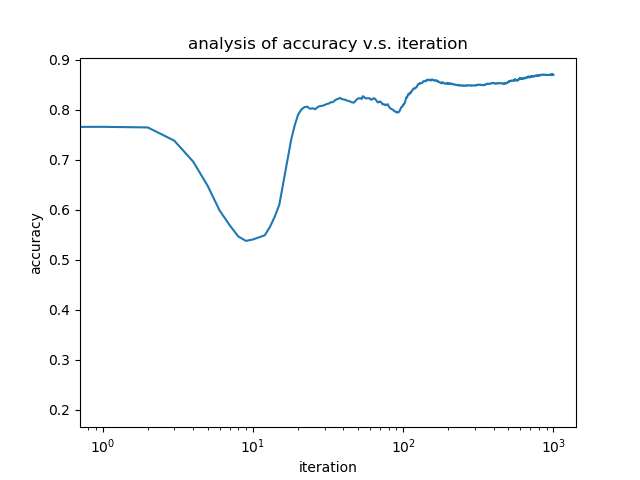
\includegraphics[width=10cm, height=13.33cm]{ana_log.png}
\caption{}
\end{figure}

\end{CJK*}
\end{document}
